% Provenance (never printed): see sources/outline_sources.md (Year 2: partial melting of the
% mantle; solidus and geotherm; decompression, hydration and heating; degree of melting;
% binary and ternary phase diagrams applied to rocks).
% Curves from figdata/bachelor-2/melting.py (Bowen 1915 diopside-anorthite, Bowen and
% Andersen 1914 forsterite-silica, Katz et al. 2003 melting of peridotite); exercise and
% problem values in the Book 4 scratch calculator calc/ch07.py.
\chapter{Fusion du manteau}\label{ch:b2:mantle-melting}

Le manteau est solide. Les ondes sismiques de cisaillement le traversent de haut
en bas, et la \omterm{def:b2:mantle-melting:peridotites}{péridotite} qu'on en remonte est une roche cristalline. Pourtant, le
long des seules dorsales océaniques, il fournit chaque année une vingtaine de
kilomètres cubes de croûte océanique neuve, chaque mètre cube étant fait d'un
liquide de fusion. Le paradoxe se dissout quand on sait que le manteau ne fond pas
parce qu'il est chauffé~: il fond parce que la pression qui s'exerce sur lui baisse,
ou parce qu'on y ajoute de l'eau. Sous une dorsale, le manteau remonte, sa pression
chute plus vite que sa température, et il croise sa courbe de fusion~; au-dessus d'une
plaque plongeante, l'eau libérée par la plaque abaisse cette courbe sous le coin de
manteau. Dans les deux cas, seule une petite fraction de la roche fond, et cette fraction,
séparée de son résidu, devient le basalte du plancher océanique et des arcs volcaniques. Ce
chapitre décrit d'abord la roche du manteau et les diagrammes de phases qui disent comment
de telles roches fondent, puis suit le manteau qui remonte sous une dorsale jusqu'à l'épaisseur de la croûte qu'il forme.
% ledger: white:crust (Book 3), data:pb2002 (Book 3), katz03:solidus

\begin{recall}
\textbf{Du volume de chimie de deuxième année}~: diagrammes de phases binaires, le
solidus et le liquidus, le point eutectique, la fusion congruente, les solutions
solides et la règle des segments inverses, selon laquelle les proportions de deux phases
coexistantes sont inversement proportionnelles à leurs distances à la composition globale.
\textbf{Des volumes de physique}~: la chaleur massique, la chaleur latente, l'entropie
et le second principe, selon lequel une transformation adiabatique réversible conserve l'entropie.
\textbf{Du volume de première année}~: les principaux minéraux formateurs de roches, l'olivine,
les pyroxènes, le grenat et le spinelle, leurs solutions solides et le nombre de Mg~; l'adiabate
du manteau, $\mathrm dT/\mathrm dz = \alpha gT/c_p$~; la croûte océanique,
\qty[uncertainty-mode=separate]{7.1 \pm 0.8}{km} d'épaisseur loin des points chauds et
d'environ \qty{20}{km} au-dessus du cœur d'un panache~; les plaques plongeantes et l'eau qu'elles
transportent. \textbf{Du \cref{ch:b2:elements-in-the-earth}}~: \omterm{def:b2:elements-in-the-earth:morb-oib}{basalte de dorsale}
(MORB), coefficients de partage et \omterm{def:b2:elements-in-the-earth:partition}{éléments incompatibles}.
\end{recall}

\section{La roche du manteau}\label{sec:b2:mantle-melting:rock}

La roche du manteau atteint la surface sous forme de fragments remontés par les \omterm{def:b2:magma-emplacement:magma}{magmas},
les xénolites, et sous forme de base de tranches de lithosphère océanique poussées sur
les continents, les ophiolites. Presque tout en est de la \omterm{def:b2:mantle-melting:peridotites}{péridotite}.
% ledger: geo:peridotite (Book 2), tulane:ocean-basins (Book 2)

\begin{definition}[Péridotites et leurs variétés]\label{def:b2:mantle-melting:peridotites}
Une \emph{péridotite}\index{péridotite} est une roche ultramafique à grains grossiers
contenant plus de \qty{40}{\percent} d'olivine, le reste étant des pyroxènes et un peu
d'un minéral alumineux (spinelle ou grenat). Une
\emph{dunite}\index{dunite} contient plus de \qty{90}{\percent} d'olivine. Au-dessous de
ce seuil, une \emph{lherzolite}\index{lherzolite} contient à la fois de l'orthopyroxène et
du clinopyroxène~; une \emph{harzburgite}\index{harzburgite} contient de l'orthopyroxène mais
presque pas de clinopyroxène~; une wehrlite contient du clinopyroxène mais presque pas
d'orthopyroxène. Les roches contenant moins de \qty{40}{\percent} d'olivine sont des pyroxénites.
\end{definition}
% ledger: bgs:ultramafic

La classification se lit sur un triangle dont les sommets sont l'olivine,
l'orthopyroxène et le clinopyroxène (figure ci-dessous)~: chaque point représente une roche,
et ses distances aux trois côtés donnent les proportions des trois
minéraux. Une composition modèle du manteau supérieur appauvri, qui fond sous
les dorsales, contient \qty{57}{\percent} d'olivine,
\qty{28}{\percent} d'orthopyroxène, \qty{13}{\percent} de clinopyroxène et
\qty{2}{\percent} de spinelle~: c'est une \omterm{def:b2:mantle-melting:peridotites}{lherzolite}.
% ledger: liang21:dmm-mode

\begin{omfigure}
\centering
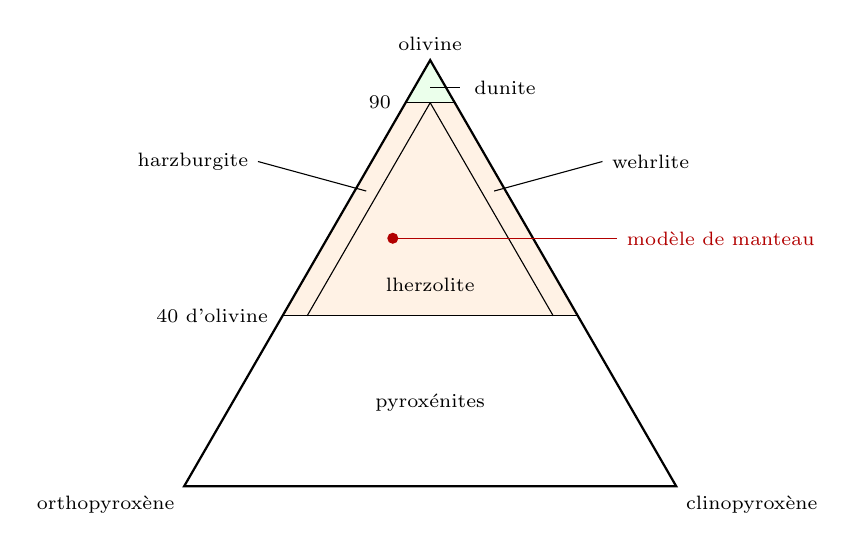
\begin{tikzpicture}[x=1.25cm, y=1.25cm, font=\scriptsize]
\coordinate (O) at (2.5,4.330); \coordinate (P) at (0,0); \coordinate (C) at (5,0);
\fill[green!8] (2.25,3.897) -- (2.75,3.897) -- (O) -- cycle;
\fill[orange!10] (1,1.732) -- (2.25,3.897) -- (2.75,3.897) -- (4,1.732) -- cycle;
\draw[thick] (O) -- (P) -- (C) -- cycle;
\draw (2.25,3.897) -- (2.75,3.897);
\draw (1,1.732) -- (4,1.732);
\draw (2.5,3.897) -- (1.25,1.732);
\draw (2.5,3.897) -- (3.75,1.732);
\node[anchor=south] at (O) {olivine};
\node[anchor=north east] at (P) {orthopyroxène};
\node[anchor=north west] at (C) {clinopyroxène};
\node[anchor=west] at (2.85,4.05) {dunite};
\draw (2.5,4.05) -- (2.8,4.05);
\node at (2.5,2.05) {lherzolite};
\draw (1.85,3.0) -- (0.75,3.3) node[anchor=east] {harzburgite};
\draw (3.15,3.0) -- (4.25,3.3) node[anchor=west] {wehrlite};
\node at (2.5,0.85) {pyroxénites};
\node[anchor=east] at (0.95,1.732) {\qty{40}{\percent} d'olivine};
\node[anchor=east] at (2.2,3.897) {\qty{90}{\percent}};
\fill[red!70!black] (2.12,2.52) circle (2pt);
\draw[red!70!black] (2.12,2.52) -- (4.4,2.52) node[anchor=west] {modèle de manteau};
\end{tikzpicture}
\par\smallskip{\small Classification des \omterm{def:b2:mantle-melting:peridotites}{péridotites} et des pyroxénites selon leurs
proportions d'olivine, d'orthopyroxène et de clinopyroxène (d'après le schéma de la
British Geological Survey). Les bandes étroites le long des deux côtés supérieurs
portent les roches presque dépourvues de clinopyroxène (\omterm{def:b2:mantle-melting:peridotites}{harzburgite}) ou dépourvues
d'orthopyroxène (wehrlite). Le point rouge figure le manteau supérieur modèle sous les
dorsales (57, 28 et \qty{13}{\percent}, renormalisés sans leurs \qty{2}{\percent} de spinelle).}
\end{omfigure}
% ledger: bgs:ultramafic, liang21:dmm-mode

Les trois \omterm{def:b2:mantle-melting:peridotites}{péridotites} ne sont pas trois types de roches indépendants~: ce sont des étapes
d'un même processus. Le clinopyroxène et le minéral alumineux sont consommés en premier
lorsqu'une \omterm{def:b2:mantle-melting:peridotites}{péridotite} fond (\cref{sec:b2:mantle-melting:decompression}), si bien qu'une
\omterm{def:b2:mantle-melting:peridotites}{lherzolite} ayant perdu un liquide s'appauvrit en eux~; après une fusion assez
poussée, elle devient une \omterm{def:b2:mantle-melting:peridotites}{harzburgite}, et une roche ayant perdu presque tout son pyroxène est une \omterm{def:b2:mantle-melting:peridotites}{dunite}.
% ledger: katz03:melting

\begin{definition}[Manteau fertile et manteau résiduel]\label{def:b2:mantle-melting:fertility}
Un \emph{manteau fertile}\index{manteau fertile} est une \omterm{def:b2:mantle-melting:peridotites}{péridotite}, typiquement une
\omterm{def:b2:mantle-melting:peridotites}{lherzolite}, qui contient encore le clinopyroxène et le minéral alumineux
dont se forme le basalte. Un \emph{manteau résiduel}\index{manteau résiduel} est la
\omterm{def:b2:mantle-melting:peridotites}{péridotite} qui reste une fois qu'un liquide en a été extrait~: plus pauvre en
clinopyroxène, en aluminium, en calcium et en \omterm{def:b2:elements-in-the-earth:partition}{éléments incompatibles}, plus riche en
olivine et à nombre de Mg plus élevé.
\end{definition}

Le \omterm{def:b2:isotope-geochemistry:reservoirs}{manteau appauvri} isotopique du \cref{ch:b2:isotope-geochemistry} est un réservoir,
défini par ses rapports isotopiques~; un \omterm{def:b2:mantle-melting:fertility}{manteau résiduel} est une roche définie par ce qu'elle a perdu.
Les deux sont liés, puisque le \omterm{def:b2:isotope-geochemistry:reservoirs}{manteau appauvri} l'est parce qu'un liquide en a été
extrait il y a longtemps, mais l'un se lit au spectromètre de masse et l'autre au
microscope.

\section{Diagrammes de phases des roches}\label{sec:b2:mantle-melting:diagrams}

Une roche est un mélange de minéraux, et elle fond sur un intervalle de températures, et non
en un point. Les diagrammes qui décrivent cela ont d'abord été mesurés sur des mélanges
de minéraux synthétiques purs, en maintenant une petite charge à une température connue jusqu'à
ce qu'elle atteigne l'équilibre, puis en la trempant et en observant au microscope le verre,
qui était du liquide, et les cristaux.

\subsection*{Un eutectique binaire~: diopside et anorthite}

Un basalte est constitué essentiellement d'un plagioclase calcique et d'un clinopyroxène, et
Bowen choisit l'anorthite et le diopside purs comme modèle le plus simple. Mélangés et chauffés,
ils forment un système eutectique ordinaire
(figure ci-dessous)~: le diopside fond à \qty{1391.5}{\celsius} et l'anorthite
à \qty{1550}{\celsius}, mais un mélange de \qty{58}{\percent} de diopside et
de \qty{42}{\percent} d'anorthite en masse fond complètement à \qty{1270}{\celsius}.
% ledger: bowen15:di-an

\begin{omfigure}
\centering
\begin{tikzpicture}
\begin{axis}[omrecord, width=0.78\linewidth, height=6cm,
  xmin=0, xmax=100, ymin=1200, ymax=1600,
  xlabel={anorthite (\unit{\percent} en masse)}, ylabel={température (\unit{\celsius})},
  y tick label style={/pgf/number format/1000 sep={}},
  tick label style={font=\scriptsize}, label style={font=\small}]
\addplot[very thick, black] table[x=x_an, y=T] {figdata/out/bachelor-2-melting-di-an-liq.dat};
\addplot[only marks, mark=*, mark size=1.6pt, blue!70!black] table[x=x_an, y=T] {figdata/out/bachelor-2-melting-di-an-data.dat};
\draw[thick] (axis cs:0,1270) -- (axis cs:100,1270);
\draw[densely dotted, red!70!black, thick] (axis cs:20,1590) -- (axis cs:20,1270);
\draw[->, red!70!black, thick] (axis cs:20,1350) -- (axis cs:41,1272);
\fill[red!70!black] (axis cs:20,1350) circle (1.6pt);
\node[font=\scriptsize] at (axis cs:55,1500) {liquide};
\node[font=\scriptsize, align=center] at (axis cs:10,1300) {diopside\\+ liquide};
\node[font=\scriptsize, align=center] at (axis cs:72,1360) {anorthite + liquide};
\node[font=\scriptsize] at (axis cs:68,1235) {diopside + anorthite};
\node[font=\scriptsize, anchor=north east] at (axis cs:41,1267) {E, \qty{1270}{\celsius}};
\node[font=\scriptsize, anchor=west, red!70!black] at (axis cs:21,1360) {premier diopside};
\end{axis}
\end{tikzpicture}
\par\smallskip{\small Le système diopside--anorthite à la pression atmosphérique, d'après
les expériences de trempe de Bowen (1915)~: températures du liquidus (points, milieux des
encadrements de trempe) et l'eutectique E. En rouge, le refroidissement d'un liquide à
\qty{20}{\percent} d'anorthite~: le diopside cristallise à partir de \qty{1350}{\celsius}, le
liquide suit le liquidus jusqu'à E, et le reste cristallise là sous forme d'un mélange des
deux minéraux.}
\end{omfigure}
% ledger: bowen15:di-an

Lu de haut en bas, le diagramme indique l'ordre de cristallisation. Un liquide à
\qty{20}{\percent} d'anorthite commence à cristalliser du diopside à
\qty{1350}{\celsius}~; le liquide, en perdant du diopside,
s'enrichit en anorthite et descend le liquidus jusqu'à l'eutectique,
où l'anorthite cristallise avec le diopside, et la
température reste à \qty{1270}{\celsius} jusqu'à ce que tout le liquide ait
disparu. Lu de bas en haut, il indique comment la roche fond~: quelles que soient les proportions
des deux minéraux, le premier liquide apparaît à \qty{1270}{\celsius} et a la
composition eutectique. C'est la première leçon pour le manteau. Le premier liquide d'une
roche n'a pas la composition de la roche~: il a celle que fixent les minéraux
dont il provient, et il apparaît à une température bien inférieure aux points de fusion de tous les minéraux.

\subsection*{Fusion incongruente~: forstérite et silice}

Certains minéraux ne fondent pas en un liquide de leur propre composition.

\begin{definition}[Fusion incongruente et point péritectique]\label{def:b2:mantle-melting:peritectic}
Un minéral présente une \emph{fusion incongruente}\index{fusion incongruente} lorsque, à la chauffe,
il se décompose en un autre solide et un liquide de composition différente,
au lieu de fondre en un liquide de sa propre composition. Sur un diagramme binaire,
le point où ce liquide coexiste avec les deux solides est un
\emph{point péritectique}\index{point péritectique}~: à la différence d'un eutectique,
il ne se situe pas entre les compositions des deux solides.
\end{definition}

L'enstatite, l'orthopyroxène magnésien \ce{MgSiO3}, fond de façon incongruente. À
pression atmosphérique, elle se décompose à \qty{1557}{\celsius} en forstérite,
\ce{Mg2SiO4}, et en un liquide un peu plus riche en silice qu'elle~; ce n'est qu'à
\qty{1577}{\celsius} que toute la forstérite est dissoute (figure ci-dessous). Bowen
et Andersen ont établi en 1914 que la décomposition donne \qty{5.5}{\percent} de
forstérite et \qty{94.5}{\percent} de liquide, comme le prévoit la règle des segments
inverses à partir des trois compositions (\cref{exo:b2:mantle-melting:6}). Plus loin vers la silice, l'enstatite et la
cristobalite fondent ensemble à un eutectique, à \qty{1543}{\celsius}.
% ledger: bowen14:mgo-sio2

\begin{omfigure}
\centering
\begin{tikzpicture}
\begin{axis}[omrecord, width=0.78\linewidth, height=6cm,
  xmin=40, xmax=66, ymin=1450, ymax=1950,
  xlabel={\ce{SiO2} (\unit{\percent} en masse)}, ylabel={température (\unit{\celsius})},
  y tick label style={/pgf/number format/1000 sep={}},
  tick label style={font=\scriptsize}, label style={font=\small}]
\addplot[very thick, black] table[x=x_sio2, y=T] {figdata/out/bachelor-2-melting-fo-sio2-liq.dat};
\addplot[very thick, black, dashed] table[x=x_sio2, y=T] {figdata/out/bachelor-2-melting-fo-sio2-fo.dat};
\draw[thick] (axis cs:42.71,1450) -- (axis cs:42.71,1890);
\draw[thick] (axis cs:42.71,1557) -- (axis cs:60.86,1557);
\draw[thick] (axis cs:59.85,1450) -- (axis cs:59.85,1557);
\draw[thick] (axis cs:59.85,1543) -- (axis cs:66,1543);
\fill (axis cs:60.86,1557) circle (1.6pt);
\fill (axis cs:64.87,1543) circle (1.6pt);
\fill (axis cs:42.71,1890) circle (1.6pt);
\node[font=\scriptsize, anchor=south west] at (axis cs:42.9,1890) {la forstérite fond, \qty{1890}{\celsius}};
\node[font=\scriptsize] at (axis cs:56,1800) {liquide};
\node[font=\scriptsize] at (axis cs:48,1680) {forstérite + liquide};
\node[font=\scriptsize] at (axis cs:51,1500) {forstérite + enstatite};
\node[font=\scriptsize, align=center] at (axis cs:63,1495) {enstatite +\\cristobalite};
\node[font=\scriptsize, anchor=south] at (axis cs:61.3,1560) {P};
\node[font=\scriptsize, anchor=south] at (axis cs:64.87,1546) {E};
\node[font=\scriptsize, anchor=north, rotate=90] at (axis cs:42.71,1650) {\ce{Mg2SiO4}};
\node[font=\scriptsize, anchor=south, rotate=90] at (axis cs:59.85,1510) {\ce{MgSiO3}};
\end{axis}
\end{tikzpicture}
\par\smallskip{\small Partie du système \ce{MgO}--\ce{SiO2} à la pression atmosphérique, d'après
Bowen et Andersen (1914). L'enstatite (\ce{MgSiO3}) fond de façon incongruente au
péritectique P, à \qty{1557}{\celsius}, en forstérite et en un liquide à
\qty{60.9}{\percent} de \ce{SiO2}~; E est l'eutectique enstatite--cristobalite,
à \qty{1543}{\celsius}. Le liquidus de la forstérite n'est mesuré qu'au voisinage de
l'enstatite~: la partie en tirets est tracée en ligne droite jusqu'au point de fusion de la forstérite.}
\end{omfigure}
% ledger: bowen14:mgo-sio2

Le péritectique est la deuxième leçon pour le manteau. Quand une \omterm{def:b2:mantle-melting:peridotites}{péridotite} fond, son
orthopyroxène ne se dissout pas simplement~: il cède de l'olivine au résidu et de la silice
au liquide. Le liquide est donc plus riche en silice que les pyroxènes, et le résidu plus riche
en olivine que la roche~: le chemin de la \omterm{def:b2:mantle-melting:peridotites}{lherzolite} à la \omterm{def:b2:mantle-melting:peridotites}{harzburgite}
puis à la \omterm{def:b2:mantle-melting:peridotites}{dunite}.

\subsection*{Trois composants~: le diagramme ternaire}

Les roches réelles comportent plus de deux minéraux. Avec trois, la composition demande un
triangle, et la température devient une troisième dimension.

\begin{definition}[Diagramme de phases ternaire, ligne cotectique, eutectique ternaire]\label{def:b2:mantle-melting:ternary}
Un \emph{diagramme de phases ternaire}\index{diagramme de phases ternaire} représente les
équilibres d'un système à trois composants à une pression donnée~: chaque point d'un
triangle représente une composition, les sommets les composants purs, et la surface du
liquidus est tracée par des courbes d'égale température ou par les domaines des minéraux
qui cristallisent en premier. Une \emph{ligne cotectique}\index{ligne cotectique} est la ligne
le long de laquelle le liquide est saturé en deux minéraux à la fois, et qui cristallise les
deux en se refroidissant. Les lignes cotectiques descendent des eutectiques binaires situés
sur les côtés du triangle et se rejoignent
à l'\emph{eutectique ternaire}\index{eutectique ternaire}, la température la plus basse
où existe un liquide, où les trois minéraux cristallisent ensemble.
\end{definition}

\begin{method}[Lire un chemin de cristallisation sur un diagramme ternaire]\label{met:b2:mantle-melting:ternary}
Repérer la composition globale $X$ dans le triangle et le domaine où elle se situe~:
le minéral de ce domaine cristallise en premier. Tant que ce seul minéral cristallise,
le liquide s'éloigne en ligne droite du sommet de ce minéral, en passant par $X$,
car retirer un composant pur ne modifie que sa proportion~; d'après la règle des segments
inverses, la fraction massique de cristaux est la distance de $X$ au liquide divisée par la
distance du sommet au liquide. Quand le liquide atteint une \omterm{def:b2:mantle-melting:ternary}{ligne cotectique}, le second minéral
se joint à la cristallisation et le liquide suit la cotectique en descendant jusqu'à l'\omterm{def:b2:mantle-melting:ternary}{eutectique
ternaire}, où cristallise le dernier liquide. Un composant qui n'entre dans aucun cristal reste
dans le liquide, si bien que sa concentration donne la fraction de liquide restante~:
$f_{\text{liquide}} = c_X/c_{\text{liquide}}$.
\end{method}

\begin{omfigure}
\centering
\begin{tikzpicture}[x=1cm, y=1cm, font=\scriptsize]
\coordinate (A) at (3,5.196); \coordinate (B) at (0,0); \coordinate (C) at (6,0);
\coordinate (eAB) at (1.2,2.078); \coordinate (eAC) at (4.65,2.338);
\coordinate (eBC) at (3.9,0); \coordinate (E) at (3.45,1.299);
\coordinate (X) at (3.0,3.118); \coordinate (L) at (3.0,1.455);
\fill[green!8] (A) -- (eAB) -- (E) -- (eAC) -- cycle;
\fill[orange!10] (B) -- (eAB) -- (E) -- (eBC) -- cycle;
\fill[blue!7] (C) -- (eAC) -- (E) -- (eBC) -- cycle;
\draw[thick] (A) -- (B) -- (C) -- cycle;
\draw[very thick, -{Stealth[length=4pt]}] (eAB) -- ($(eAB)!0.55!(E)$);
\draw[very thick] ($(eAB)!0.5!(E)$) -- (E);
\draw[very thick, -{Stealth[length=4pt]}] (eAC) -- ($(eAC)!0.55!(E)$);
\draw[very thick] ($(eAC)!0.5!(E)$) -- (E);
\draw[very thick, -{Stealth[length=4pt]}] (eBC) -- ($(eBC)!0.55!(E)$);
\draw[very thick] ($(eBC)!0.5!(E)$) -- (E);
\draw[red!70!black, thick, dashed] (A) -- (X);
\draw[red!70!black, very thick, -{Stealth[length=4pt]}] (X) -- (L);
\draw[red!70!black, very thick, -{Stealth[length=4pt]}] (L) -- ($(L)!0.85!(E)$);
\fill[red!70!black] (X) circle (2pt); \fill[red!70!black] (L) circle (1.6pt);
\fill (E) circle (2pt);
\node[anchor=south] at (A) {A}; \node[anchor=north east] at (B) {B};
\node[anchor=north west] at (C) {C};
\node[anchor=west, red!70!black] at (3.1,3.2) {$X$};
\node[anchor=north east, red!70!black] at (2.95,1.42) {$L_1$};
\node[anchor=north west] at (3.5,1.25) {E};
\node[anchor=east] at (eAB) {$e_{AB}$}; \node[anchor=west] at (eAC) {$e_{AC}$};
\node[anchor=north] at (eBC) {$e_{BC}$};
\node at (2.35,2.75) {domaine A}; \node at (1.55,0.7) {domaine B}; \node at (4.9,0.7) {domaine C};
\end{tikzpicture}
\par\smallskip{\small Un système \omterm{def:b2:mantle-melting:ternary}{eutectique ternaire} (schéma). Chaque domaine contient
les liquides à partir desquels son minéral cristallise en premier~; les \omterm{def:b2:mantle-melting:ternary}{lignes cotectiques} (flèches
vers les températures décroissantes) partent des eutectiques binaires $e$ jusqu'à
l'\omterm{def:b2:mantle-melting:ternary}{eutectique ternaire} E. Un liquide $X$ dans le domaine A cristallise A, et s'éloigne du
sommet A jusqu'à rencontrer la cotectique A--B en $L_1$~; A et B cristallisent alors
ensemble jusqu'à E, où C les rejoint (\cref{exo:b2:mantle-melting:11}).}
\end{omfigure}

Les systèmes de trois minéraux formateurs de roches se lisent de la même manière. Les règles qui fixent le nombre de phases pouvant coexister,
et les surfaces d'énergie libre à partir desquelles de tels diagrammes sont calculés, relèvent du
volume de troisième année de cette série.

\section{Solidus, adiabate et trois façons de fondre}\label{sec:b2:mantle-melting:solidus}

La \omterm{def:b2:mantle-melting:peridotites}{péridotite} du manteau possède un solidus, température à laquelle apparaît son premier
liquide, et un liquidus bien au-dessus. Les deux augmentent avec la pression. Les expériences
sur des \omterm{def:b2:mantle-melting:peridotites}{péridotites} naturelles, compilées et ajustées par Katz, Spiegelman et Langmuir en 2003, donnent
pour le solidus sec
\[
  T_{\mathrm{s}}(P) = 1085.7 + 132.9\,P - 5.1\,P^2
\]
(en degrés Celsius, $P$ en gigapascals)~: \qty{1086}{\celsius} en surface,
\qty{1331}{\celsius} à \qty{2}{GPa}. À profondeur égale, le manteau est plus chaud ou
plus froid que cela selon l'endroit où il se trouve, et pour comparer les manteaux on retire
l'effet de la profondeur.
% ledger: katz03:solidus

\begin{definition}[Température potentielle du manteau]\label{def:b2:mantle-melting:tp}
La \emph{température potentielle du manteau}\index{température potentielle du manteau} $T_p$
est la température qu'aurait une parcelle de manteau en convection si on la ramenait
à la surface le long de l'adiabate du manteau, sans échange de chaleur et
sans fusion.
\end{definition}

Le long de l'adiabate $\mathrm dT/\mathrm dP = \alpha T/(\rho c_p)$, la forme en
pression du gradient $\alpha gT/c_p$ rappelé plus haut, puisque $\mathrm dP = \rho
g\,\mathrm dz$. Avec $\alpha = \qty{4e-5}{K^{-1}}$, $\rho = \qty{3300}{kg/m^3}$
et $c_p = \qty{1000}{J/(kg.K)}$, il vaut environ \qty{20}{K} par gigapascal, un gigapascal
représentant \qty{30.9}{km} de manteau (\cref{exo:b2:mantle-melting:3}). Le volume de première année
attribuait au manteau une température potentielle d'environ \qty{1350}{\celsius}, d'après la physique des
minéraux~; les estimations pétrologiques pour le manteau sous les dorsales vont de 1280 à
\qty{1400}{\celsius}.
% ledger: katz03:thermo, katsura:adiabat (Book 3), herzberg:tp (Book 3)

\begin{proposition}[Début de la fusion par décompression]\label{prop:b2:mantle-melting:onset}
Un manteau de température potentielle $T_p$ qui remonte le long de l'adiabate $T = T_p + GP$ ($G$
constante) commence à fondre à la pression $P_0$ où l'adiabate rencontre le
solidus $T_{\mathrm s}(P) = a_1 + a_2P + a_3P^2$, la plus petite racine de
\[
  -a_3P^2 + (G - a_2)P + (T_p - a_1) = 0 .
\]
Un manteau plus chaud de $\Delta T_p$ commence à fondre plus profondément, de $\Delta P_0 \approx
\Delta T_p/(T_{\mathrm s}'(P_0) - G)$.
\end{proposition}

\begin{proof}
En profondeur, l'adiabate est plus froide que le solidus, car le solidus monte plus
rapidement ($T_{\mathrm
s}' \approx \qty{110}{K/GPa}$ contre $G \approx 20$). Les deux courbes se croisent là où
$T_p + GP = a_1 + a_2P + a_3P^2$, ce qui se ramène au trinôme. En dérivant
$T_p + GP_0 = T_{\mathrm s}(P_0)$ on obtient $\mathrm dT_p = (T_{\mathrm s}'(P_0) -
G)\,\mathrm dP_0$.
\end{proof}

Pour $T_p = \qty{1350}{\celsius}$, le début de la fusion se situe à \qty{2.66}{GPa}, soit environ
\qty{82}{km} de profondeur, à \qty{1403}{\celsius}~; chaque \qty{10}{\celsius} de température
potentielle la déplace d'environ \qty{0.12}{GPa}, soit \qty{3.6}{km}. La figure ci-dessous
montre le solidus et les adiabates.

\begin{omfigure}
\centering
\begin{tikzpicture}
\begin{axis}[omrecord, width=0.8\linewidth, height=7cm,
  xmin=850, xmax=2000, ymin=0, ymax=6, y dir=reverse,
  xlabel={température (\unit{\celsius})}, ylabel={pression (\unit{GPa})},
  x tick label style={/pgf/number format/1000 sep={}},
  axis y line*=left,
  legend style={font=\scriptsize, at={(0.5,-0.2)}, anchor=north, legend columns=3},
  tick label style={font=\scriptsize}, label style={font=\small}]
\addplot[very thick, black] table[x=Ts, y=P_GPa] {figdata/out/bachelor-2-melting-pt.dat};
\addlegendentry{solidus sec}
\addplot[thick, black, densely dotted] table[x=Tl, y=P_GPa] {figdata/out/bachelor-2-melting-pt.dat};
\addlegendentry{liquidus de la lherzolite}
\addplot[thick, black, dashed] table[x=Tq, y=P_GPa] {figdata/out/bachelor-2-melting-pt.dat};
\addlegendentry{liquidus}
\addplot[thick, blue!70!black, dashdotted] table[x=wetsat, y=P_GPa] {figdata/out/bachelor-2-melting-pt.dat};
\addlegendentry{solidus saturé en eau}
\addplot[thick, red!70!black] table[x=ad1350, y=P_GPa] {figdata/out/bachelor-2-melting-pt.dat};
\addlegendentry{adiabates, $T_p$ = 1300, 1350, \qty{1450}{\celsius}}
\addplot[thin, red!70!black] table[x=ad1300, y=P_GPa] {figdata/out/bachelor-2-melting-pt.dat};
\addplot[thin, red!70!black] table[x=ad1450, y=P_GPa] {figdata/out/bachelor-2-melting-pt.dat};
\addplot[only marks, mark=*, mark size=2pt, red!70!black] table[x=T0, y=P0] {figdata/out/bachelor-2-melting-onset.dat};
\end{axis}
\begin{axis}[width=0.8\linewidth, height=7cm, xmin=850, xmax=2000,
  ymin=0, ymax=185.34, y dir=reverse, axis y line*=right, axis x line=none,
  ylabel={profondeur (\unit{km})}, tick label style={font=\scriptsize}, label style={font=\small}]
\end{axis}
\end{tikzpicture}
\par\smallskip{\small Courbes de fusion de la \omterm{def:b2:mantle-melting:peridotites}{péridotite} sèche et solidus saturé en eau
d'après la paramétrisation de Katz et ses collaborateurs (2003), avec des adiabates pleines
pour trois températures potentielles~; les points marquent le début de la fusion,
\qty{2.08}{GPa} pour \qty{1300}{\celsius}, \qty{2.66}{GPa} pour
\qty{1350}{\celsius} et \qty{4.00}{GPa} pour \qty{1450}{\celsius}. Entre le
solidus et le liquidus de la \omterm{def:b2:mantle-melting:peridotites}{lherzolite}, la roche fond tout en conservant son
clinopyroxène. Échelle de profondeur pour un manteau de \qty{3300}{kg/m^3}.}
\end{omfigure}
% ledger: katz03:solidus, katz03:water, katz03:thermo

Le diagramme montre les trois façons de porter une roche au-dessus de son solidus.

\begin{definition}[Fusion partielle, fusion par décompression et fusion hydratée]\label{def:b2:mantle-melting:melting}
\emph{Fusion partielle}\index{fusion partielle} est la fusion d'une fraction d'une
roche, entre son solidus et son liquidus. \emph{Fusion par
décompression}\index{fusion par décompression} est la fusion partielle d'une roche qui monte,
et donc perd de la pression, plus vite qu'elle ne se refroidit, jusqu'à croiser son solidus.
\emph{Fusion hydratée}\index{fusion hydratée}\index{fusion par flux|see{fusion hydratée}},
ou fusion par apport d'eau, est la fusion partielle provoquée par l'ajout d'un volatil,
principalement de l'eau, qui abaisse le solidus sous la température de la roche. Le troisième
mode, chauffer une roche au-dessus de son solidus à pression constante, exige une source
de chaleur extérieure, comme un \omterm{def:b2:magma-emplacement:magma}{magma} chaud.
\end{definition}

Le chauffage est le mode le moins efficace dans le manteau, qui conduit lentement la chaleur~; dans
la croûte, la chaleur d'un \omterm{def:b2:magma-emplacement:magma}{magma} basaltique peut fondre les roches qui l'entourent
(\cref{ch:b2:crustal-melting}). La décompression alimente les dorsales et les points chauds~;
la \omterm{def:b2:mantle-melting:melting}{fusion hydratée} alimente les arcs volcaniques.

\section{Fusion par décompression sous une dorsale}\label{sec:b2:mantle-melting:decompression}

Une fois que le manteau qui monte a franchi son solidus, il continue de monter, et la question
devient celle de la quantité de liquide qu'il produit.

\begin{definition}[Taux de fusion]\label{def:b2:mantle-melting:fraction}
Le \emph{taux de fusion}\index{taux de fusion} $F$ d'une roche partiellement fondue est
la masse de liquide qu'elle a produite divisée par sa masse initiale. Entre le solidus
($F = 0$) et le liquidus ($F = 1$), la température à la surface de fusion est une
fonction $T(P, F)$.
\end{definition}

La fusion consomme de la chaleur~: la chaleur latente, $T\Delta S$ par kilogramme de liquide, où
$\Delta S$ est l'entropie de fusion. Une parcelle qui monte n'échange pas de chaleur avec son
environnement, si bien que la chaleur latente est prélevée sur sa propre température, et elle
suit un chemin d'entropie constante situé entre le solidus et le liquidus.

\begin{proposition}[Productivité de fusion isentropique]\label{prop:b2:mantle-melting:productivity}
Pour un manteau qui monte sans échange de chaleur, de chaleur massique $c_p$, de dilatation
thermique $\alpha$, de masse volumique $\rho$ et d'entropie de fusion $\Delta S$, la
\emph{productivité de fusion}\index{productivité de fusion}, c'est-à-dire le liquide produit par unité de
baisse de pression, vaut
\[
  -\frac{\mathrm dF}{\mathrm dP} =
  \frac{\dfrac{c_p}{T}\Big(\dfrac{\partial T}{\partial P}\Big)_F - \dfrac{\alpha}{\rho}}
       {\Delta S + \dfrac{c_p}{T}\Big(\dfrac{\partial T}{\partial F}\Big)_P}\,,
\]
avec $T$ en kelvins.
\end{proposition}

\begin{proof}
L'entropie spécifique de la roche partiellement fondue varie de $\mathrm ds = c_p\,
\mathrm dT/T - (\alpha/\rho)\,\mathrm dP + \Delta S\,\mathrm dF$~: les deux premiers
termes sont ceux d'un solide (le second est une relation de Maxwell, rappelée des
volumes de physique), le troisième est l'entropie gagnée par la masse $\mathrm dF$ qui
fond. Une montée adiabatique réversible conserve $\mathrm ds = 0$. Sur la
surface de fusion $\mathrm dT = (\partial T/\partial P)_F\,\mathrm dP + (\partial
T/\partial F)_P\,\mathrm dF$. En substituant,
\[
  \Big[\frac{c_p}{T}\Big(\frac{\partial T}{\partial P}\Big)_F - \frac{\alpha}{\rho}\Big]\mathrm dP
  + \Big[\Delta S + \frac{c_p}{T}\Big(\frac{\partial T}{\partial F}\Big)_P\Big]\mathrm dF = 0,
\]
qui est le résultat.
\end{proof}

Le numérateur est l'excès de la pente des courbes de fusion sur celle de l'adiabate, le
moteur~; le dénominateur regroupe la chaleur latente et la chaleur nécessaire pour élever la
température de la roche qui fond le long de l'intervalle de fusion, les freins. Avec les
paramètres de Katz et ses collaborateurs, $\Delta S = \qty{300}{J/(kg.K)}$, et un \omterm{def:b2:mantle-melting:fraction}{taux de
fusion} qui croît linéairement entre le solidus et le liquidus de la \omterm{def:b2:mantle-melting:peridotites}{lherzolite}, la
productivité à \qty{2}{GPa} vaut environ \qty{11}{\percent} par gigapascal
(\cref{exo:b2:mantle-melting:8})~: chaque kilomètre de montée fond environ un tiers de pour cent de la
roche. Leur fonction de fusion ajustée, qui fait que le premier pour cent de liquide apparaît
lentement, donne un peu moins en moyenne, environ \qty{9}{\percent} par gigapascal
depuis le début de la fusion jusqu'à la surface, pour $T_p = \qty{1350}{\celsius}$. La productivité
chute lorsque le clinopyroxène est épuisé, après des \omterm{def:b2:mantle-melting:fraction}{taux de fusion}
de $M_{\mathrm{cpx}}/(0.50 + 0.08P)$ dans leur modèle, soit environ 25 à \qty{30}{\percent} pour
un manteau à 13 à \qty{15}{\percent} de clinopyroxène~: un résidu de \omterm{def:b2:mantle-melting:peridotites}{harzburgite} fond
à contrecœur.
% ledger: katz03:melting, katz03:thermo

\begin{omfigure}
\centering
\begin{tikzpicture}
\begin{axis}[omrecord, width=0.62\linewidth, height=6.4cm,
  xmin=0, xmax=0.36, ymin=0, ymax=130, y dir=reverse,
  xlabel={taux de fusion $F$}, ylabel={profondeur (\unit{km})},
  xtick={0,0.1,0.2,0.3},
  legend style={font=\scriptsize, at={(0.98,0.02)}, anchor=south east},
  tick label style={font=\scriptsize}, label style={font=\small}]
\addplot[thick, blue!70!black] table[x=F1300, y=z_km] {figdata/out/bachelor-2-melting-column.dat};
\addlegendentry{$T_p = \qty{1300}{\celsius}$}
\addplot[very thick, black] table[x=F1350, y=z_km] {figdata/out/bachelor-2-melting-column.dat};
\addlegendentry{$T_p = \qty{1350}{\celsius}$}
\addplot[thick, red!70!black, dashed] table[x=F1450, y=z_km] {figdata/out/bachelor-2-melting-column.dat};
\addlegendentry{$T_p = \qty{1450}{\celsius}$}
\end{axis}
\end{tikzpicture}
\par\smallskip{\small \omterm{def:b2:mantle-melting:fraction}{Taux de fusion} d'une colonne de \omterm{def:b2:mantle-melting:peridotites}{péridotite} sèche qui monte sans
échange de chaleur, depuis le début de la fusion jusqu'à la surface, calculé en conservant
l'entropie avec la fonction de fusion de Katz et ses collaborateurs (2003), pour une roche
à \qty{15}{\percent} de clinopyroxène. À \qty{1450}{\celsius}, le clinopyroxène est épuisé
vers \qty{25}{km}, et la courbe se raidit.}
\end{omfigure}
% ledger: katz03:melting, katz03:thermo

Le liquide ne reste pas là où il se forme. À environ \qty{2900}{kg/m^3} il est plus léger que la
\omterm{def:b2:mantle-melting:peridotites}{péridotite} solide, \qty{3300}{kg/m^3}, si bien qu'il se sépare de son résidu et monte à travers
celui-ci~; sous une dorsale, il est rassemblé vers l'axe.
La croûte se construit à partir des liquides d'une région entière du manteau.
% ledger: katz03:thermo

\begin{proposition}[Croûte d'une région de fusion triangulaire]\label{prop:b2:mantle-melting:triangle}
Sous une dorsale qui s'écarte à la demi-vitesse $U$, le manteau monte verticalement à la
vitesse $U$ à travers une région de fusion triangulaire de hauteur $H$, dont le sommet est sous
l'axe et les côtés à \ang{45}, puis en sort horizontalement à la vitesse $U$ par ses côtés~;
le \omterm{def:b2:mantle-melting:fraction}{taux de fusion} croît linéairement de $0$ à la base jusqu'à $F_{\max}$ au sommet, tout le liquide
est extrait vers la croûte, et manteau et
croûte ont la même masse volumique. Alors la croûte est
\[
  h_c = \int_0^H F(z)\,\mathrm dz = \tfrac12 F_{\max}H
\]
épaisse, et le liquide agrégé a pour \omterm{def:b2:mantle-melting:fraction}{taux de fusion} moyen $F_{\max}/2$.
\end{proposition}

\begin{proof}
Mesurons $x$ depuis l'axe et la hauteur $y$ au-dessus de la base. Le manteau entre par la base
en $|x| \le H$ et monte jusqu'à rencontrer un côté, en $y = H - |x|$, en ayant fondu jusqu'à
$F = F_{\max}(H - |x|)/H$. Par unité de longueur de dorsale et par unité de temps, le liquide produit vaut
$\int_{-H}^{H} U F\,\mathrm dx = 2UF_{\max}\int_0^H (1 - x/H)\,\mathrm dx =
UF_{\max}H$. La croûte sort des deux côtés à la vitesse $U$~: $2Uh_c = UF_{\max}H$.
Le manteau traité vaut $2UH$, donc le \omterm{def:b2:mantle-melting:fraction}{taux de fusion} moyen est $UF_{\max}H/(2UH) =
F_{\max}/2$. Enfin $\int_0^H F_{\max}\,y/H\,\mathrm dy = F_{\max}H/2$.
\end{proof}

Le résultat ne dépend pas de la vitesse d'écartement, comme on l'observe (le volume de
première année). Pour $T_p = \qty{1350}{\celsius}$, la colonne de la figure ci-dessus, avec son
départ lent, donne $\int F\,\mathrm dz = \qty{9.0}{km}$ de croûte, un peu plus que les
\qty{7.1}{km} mesurés~; un manteau \qty{50}{\celsius} plus froid donne
\qty{5.5}{km}, et un manteau \qty{100}{\celsius} plus chaud \qty{19}{km}, proche des
\qty{20}{km} sous le cœur d'un panache (figure ci-dessous). L'épaisseur de la croûte est un
thermomètre, et un thermomètre sensible~: puisque $h_c \propto P_0^2$ lorsque la productivité est
constante, dix degrés la modifient d'environ un dixième (problème du week-end).
% ledger: white:crust (Book 3)

\begin{omfigure}
\centering
\begin{tikzpicture}[x=1cm, y=1cm, font=\scriptsize]
\fill[blue!8] (-5.5,0.6) rectangle (5.5,0);
\fill[brown!35] (-5.5,0) -- (5.5,0) -- (5.5,-0.35) -- (-5.5,-0.35) -- cycle;
\fill[orange!25] (0,-0.45) -- (-3.6,-4.05) -- (3.6,-4.05) -- cycle;
\draw[densely dashed, thick] (-5.5,-4.05) -- (5.5,-4.05);
\node[anchor=north east] at (5.5,-4.55) {solidus franchi~: début de la fusion, profondeur $z_0$};
\foreach \s in {1,-1} {
  \draw[->, thick] (\s*0.4,0.35) -- (\s*1.6,0.35);
  \draw[gray, -{Stealth[length=3pt]}] (\s*1.8,-4.5) -- (\s*1.8,-2.45) .. controls (\s*1.8,-2.1) and (\s*2.1,-1.95) .. (\s*2.8,-1.95) -- (\s*5.3,-1.95);
  \draw[gray, -{Stealth[length=3pt]}] (\s*3.1,-4.5) -- (\s*3.1,-3.75) .. controls (\s*3.1,-3.4) and (\s*3.4,-3.25) .. (\s*4.1,-3.25) -- (\s*5.3,-3.25);
}
\draw[red!70!black, -{Stealth[length=3pt]}, thick] (-1.2,-3.0) -- (-0.3,-1.0);
\draw[red!70!black, -{Stealth[length=3pt]}, thick] (1.2,-3.0) -- (0.3,-1.0);
\draw[red!70!black, -{Stealth[length=3pt]}, thick] (0,-2.3) -- (0,-0.9);
\node[anchor=south] at (0,0.6) {axe de la dorsale};
\node[anchor=west] at (1.7,0.35) {plaque, vitesse $U$};
\node[anchor=west] at (-5.4,-0.2) {croûte, $h_c$};
\node[align=center, inner sep=1pt] at (0,-3.3) {région de fusion};
\node[anchor=west, align=left] at (3.2,-2.55) {lignes de courant\\du manteau};
\node[anchor=east, align=right, red!70!black] at (-2.0,-2.6) {le liquide gagne\\l'axe};
\end{tikzpicture}
\par\smallskip{\small Région de fusion triangulaire sous une dorsale (schéma, non
à l'échelle~; en réalité $z_0$ vaut dix fois l'épaisseur de la croûte). Le manteau qui monte
sous l'axe franchit son solidus en $z_0$, fond en montant, et cesse de fondre
lorsque son écoulement devient horizontal sous les plaques en mouvement~; le liquide remonte
vers l'axe et construit la croûte.}
\end{omfigure}

\begin{omfigure}
\centering
\begin{tikzpicture}
\begin{axis}[omrecord, width=0.72\linewidth, height=5.6cm,
  xmin=1250, xmax=1550, ymin=0, ymax=32,
  xlabel={température potentielle du manteau $T_p$ (\unit{\celsius})},
  ylabel={croûte formée (\unit{km})},
  x tick label style={/pgf/number format/1000 sep={}},
  tick label style={font=\scriptsize}, label style={font=\small}]
\fill[blue!12] (axis cs:1250,6.3) rectangle (axis cs:1550,7.9);
\fill[red!12] (axis cs:1250,19) rectangle (axis cs:1550,21);
\addplot[very thick, black] table[x=Tp, y=h_km] {figdata/out/bachelor-2-melting-crust.dat};
\node[font=\scriptsize, anchor=west, blue!60!black] at (axis cs:1400,7.1) {dorsales normales, $7.1 \pm 0.8$};
\node[font=\scriptsize, anchor=east, red!60!black] at (axis cs:1440,20) {au-dessus d'un panache, $20 \pm 1$};
\end{axis}
\end{tikzpicture}
\par\smallskip{\small Épaisseur de la croûte formée par une région de fusion triangulaire,
$\int F\,\mathrm dz$ le long de l'axe, en fonction de la \omterm{def:b2:mantle-melting:tp}{température potentielle du
manteau} (colonnes comme dans la figure ci-dessus), comparée à l'épaisseur sismique de la
croûte océanique normale et de la croûte au-dessus du cœur d'un panache (bandes).}
\end{omfigure}
% ledger: katz03:melting, white:crust (Book 3)

\section{Fusion hydratée au-dessus d'une plaque plongeante}\label{sec:b2:mantle-melting:flux}

À une zone de subduction, le coin de manteau ne monte pas~; il est entraîné vers le bas le long
de la plaque plongeante. C'est l'eau qui le fait fondre. La plaque transporte l'eau vers le bas dans ses
minéraux et la libère à mesure qu'ils se décomposent sous l'effet de la pression et de la température
(le volume de première année)~; l'eau monte dans le coin chaud au-dessus. L'eau se dissout dans le \omterm{def:b2:magma-emplacement:magma}{liquide silicaté}, et un
liquide qui en contient est stable à plus basse température. Dans la paramétrisation de
Katz et ses collaborateurs, $X$ pour cent d'eau dissoute dans le liquide abaisse le solidus de
\[
  \Delta T = 43\,X^{0.75} \quad (\unit{\celsius}),
\]
\qty{43}{\celsius} pour \qty{1}{\percent}, \qty{144}{\celsius} pour
\qty{5}{\percent}, jusqu'à la quantité qui sature le liquide, nulle à pression atmosphérique,
environ \qty{13}{\percent} à \qty{1}{GPa}, et qui croît avec la
pression. Le solidus saturé en eau est la courbe bleue de la figure du solidus~:
voisin de \qty{920}{\celsius} entre 1 et \qty{2}{GPa}, environ \qty{300}{\celsius} à
\qty{400}{\celsius} sous le solidus sec (\cref{exo:b2:mantle-melting:12}).
% ledger: katz03:water, katz03:solidus

L'eau est incompatible~: elle entre dans le liquide bien plus facilement que dans les minéraux,
avec un coefficient de partage d'environ 0.01. Même un manteau contenant une centaine de
parties par million d'eau produit donc un premier liquide contenant environ un pour cent d'eau, qui
abaisse son solidus d'environ \qty{50}{\celsius}, si bien que la fusion
commence plus profondément que dans un manteau sec, et qu'il se forme une longue traîne de petites
fractions fondues (\cref{exo:b2:mantle-melting:9}). Au-dessus d'une plaque, l'apport d'eau est bien plus
grand, et le coin fond là où sa température dépasse le solidus hydraté~: les \omterm{def:b2:magma-emplacement:magma}{magmas} des arcs naissent
hydratés.
% ledger: katz03:water

\section{Degré de fusion et magmas primaires}\label{sec:b2:mantle-melting:primary}

\begin{definition}[Magma primaire]\label{def:b2:mantle-melting:primary}
Un \emph{magma primaire}\index{magma primaire} est un liquide dont la composition n'a pas
changé depuis qu'il a quitté sa source~: il est en équilibre avec le \omterm{def:b2:mantle-melting:fertility}{manteau résiduel},
et n'a ni cristallisé de minéraux ni réagi avec les roches sur son chemin vers la surface.
\end{definition}

Un \omterm{def:b2:magma-emplacement:magma}{magma} qui cristallise des minéraux en remontant, ou qui se mélange à d'autres, n'est plus
primaire~; la manière dont il évolue ensuite fait l'objet du
\cref{ch:b2:magmatic-differentiation}. Un \omterm{def:b2:mantle-melting:primary}{magma primaire} garde la trace de sa source~: son
\omterm{def:b2:mantle-melting:fraction}{taux de fusion}, car un faible degré de fusion concentre les \omterm{def:b2:elements-in-the-earth:partition}{éléments incompatibles}
dans le liquide (\cref{ch:b2:elements-in-the-earth}), et la pression à laquelle il s'est
équilibré pour la dernière fois avec le résidu. La répartition des \omterm{def:b2:elements-in-the-earth:trace}{éléments en traces} entre
liquide et résidu, lors de la fusion à l'équilibre ou de la fusion fractionnée, est modélisée dans le volume de troisième année. Le
résidu, quant à lui, est la \omterm{def:b2:mantle-melting:peridotites}{harzburgite} et la \omterm{def:b2:mantle-melting:peridotites}{péridotite} que l'on trouve à la base des
ophiolites.
% ledger: tulane:ocean-basins (Book 2)

\begin{inthefield}[Lire le manteau à la surface]
\begin{minipage}[t]{0.6\linewidth}\vspace{0pt}
Les géologues rencontrent le manteau sous deux formes. Les xénolites du manteau, nodules de
\omterm{def:b2:mantle-melting:peridotites}{péridotite} verte dans les basaltes et les kimberlites, ont été arrachés aux parois du conduit
et remontés en quelques jours ou semaines, trop vite pour perdre les minéraux qu'ils avaient en
profondeur. Les ophiolites exposent le manteau sous une section de croûte océanique, sa
\omterm{def:b2:mantle-melting:peridotites}{harzburgite} et d'autres \omterm{def:b2:mantle-melting:peridotites}{péridotites} à la base de la séquence. Là, les géologues
cartographient les \omterm{def:b2:mantle-melting:peridotites}{péridotites} et la \omterm{def:b2:mantle-melting:peridotites}{dunite} parmi elles, les échantillonnent le long de traverses, et
mesurent au laboratoire les proportions des minéraux, leurs compositions et
les \omterm{def:b2:elements-in-the-earth:trace}{éléments en traces} des résidus~; chaque échantillon est placé sur le triangle de
classification et sur les chemins de fusion de ce chapitre.
\end{minipage}\hfill
\begin{minipage}[t]{0.36\linewidth}\vspace{0pt}
\centering
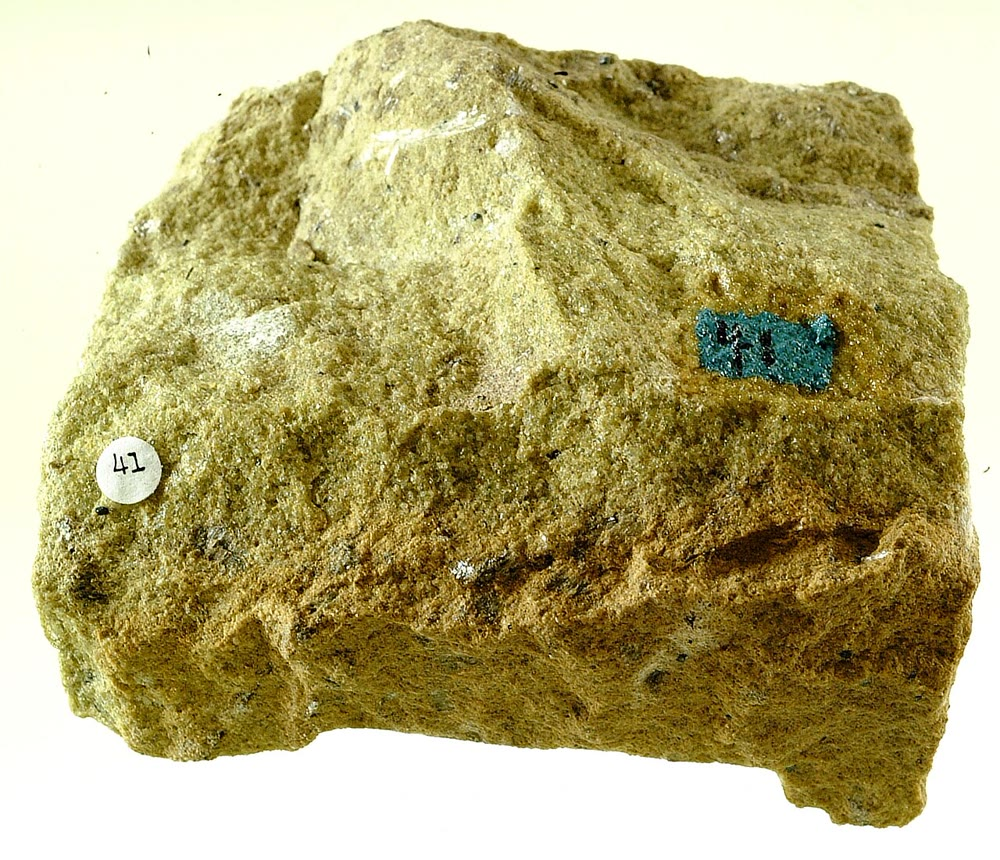
\includegraphics[width=\linewidth]{images/book4/b2-dunite.jpg}
\par\smallskip{\scriptsize Une \omterm{def:b2:mantle-melting:peridotites}{dunite}, presque entièrement faite d'olivine, avec de petits
grains noirs de chromite~; l'échantillon mesure \qty{8.5}{cm} de large (Mike Davis, CC0).}
\end{minipage}
\end{inthefield}
% ledger: casetta23:kimberlite, tulane:ocean-basins (Book 2), bgs:ultramafic

\section{Exercices}

\begin{exercise}[$\star$]\label{exo:b2:mantle-melting:1}
Nommer chaque roche d'après ses proportions d'olivine, d'orthopyroxène et de clinopyroxène
(en pour cent)~: (a) 93, 5, 2~; (b) 75, 25, 0~; (c) 60, 27, 13~; (d) 30, 45, 25. (e) Donner
le nom du manteau supérieur modèle (57, 28, 13 et \qty{2}{\percent} de spinelle) après
renormalisation de ses trois silicates à \qty{100}{\percent}.
\end{exercise}
% ledger: bgs:ultramafic, liang21:dmm-mode

\begin{exercise}[$\star$]\label{exo:b2:mantle-melting:2}
Sur le diagramme diopside--anorthite, un liquide à \qty{60}{\percent} d'anorthite
se refroidit. (a) À quelle température commence-t-il à cristalliser, et quel minéral
se forme~? (b) À quelle température apparaît le second minéral, et quelle est alors
la composition du liquide~? (c) Quelle est la composition du premier liquide lorsqu'une
roche à \qty{80}{\percent} de diopside et \qty{20}{\percent} d'anorthite est chauffée,
et à quelle température apparaît-il~?
\end{exercise}
% ledger: bowen15:di-an

\begin{exercise}[$\star$]\label{exo:b2:mantle-melting:3}
(a) Calculer le gradient adiabatique $\alpha T/(\rho c_p)$ en kelvins par gigapascal
pour $T_p = \qty{1350}{\celsius}$, $\alpha = \qty{4.0e-5}{K^{-1}}$, $\rho =
\qty{3300}{kg/m^3}$, $c_p = \qty{1000}{J/(kg.K)}$. (b) Combien de kilomètres de
manteau correspondent à un gigapascal ($g = \qty{9.81}{m/s^2}$)~? Convertir le gradient en kelvins
par kilomètre et le comparer à un gradient géothermique typique près de la surface,
d'environ \qty{30}{K/km}.
\end{exercise}
% ledger: katz03:thermo, earle:settings (Book 2)

\begin{exercise}[$\star$]\label{exo:b2:mantle-melting:4}
(a) Calculer le solidus sec de la \omterm{def:b2:mantle-melting:peridotites}{péridotite} à 0, 1, 2 et \qty{3}{GPa}. (b) De combien de degrés
monte-t-il par gigapascal au voisinage de \qty{2}{GPa}~? (c) Expliquer en une phrase pourquoi un manteau à
\qty{1400}{\celsius} à \qty{3}{GPa} est solide, et le même manteau porté à \qty{2}{GPa} sans
échange de chaleur est partiellement fondu.
\end{exercise}
% ledger: katz03:solidus

\begin{exercise}[$\star\star$]\label{exo:b2:mantle-melting:5}
Un liquide à \qty{70}{\percent} de diopside et \qty{30}{\percent} d'anorthite se refroidit.
(a) Estimer sa température de liquidus par interpolation entre le liquidus à
\qty{20}{\percent} d'anorthite (\qty{1350}{\celsius}) et à \qty{40}{\percent}
(\qty{1277.5}{\celsius}). (b) Quel minéral cristallise en premier~? (c) Quelle fraction
massique du système a cristallisé lorsque le liquide atteint l'eutectique~?
(d) Quelles sont les proportions de diopside et d'anorthite dans la roche finale~?
\end{exercise}
% ledger: bowen15:di-an

\begin{exercise}[$\star\star$]\label{exo:b2:mantle-melting:6}
(a) Calculer le pourcentage massique de \ce{SiO2} dans la forstérite \ce{Mg2SiO4} et dans
l'enstatite \ce{MgSiO3} ($M_{\ce{MgO}} = \qty{40.30}{g/mol}$, $M_{\ce{SiO2}} =
\qty{60.08}{g/mol}$). (b) Bowen et Andersen ont trouvé que le liquide péritectique contient
\qty{97.5}{\percent} de \ce{MgSiO3} et \qty{2.5}{\percent} de \ce{SiO2}~: quelle est sa
teneur en silice~? (c) Utiliser la règle des segments inverses pour calculer la fraction massique de forstérite
formée lorsque l'enstatite fond au péritectique, et la comparer à leur
\qty{5.5}{\percent}. (d) Qu'implique cela pour la teneur en silice d'un liquide de
\omterm{def:b2:mantle-melting:peridotites}{péridotite}, comparée à celle de son orthopyroxène~?
\end{exercise}
% ledger: bowen14:mgo-sio2

\begin{exercise}[$\star\star$]\label{exo:b2:mantle-melting:7}
Avec l'adiabate $T = T_p + 20P$ et le solidus sec du texte, calculer la
pression et la profondeur ($\qty{30.9}{km}$ par gigapascal) auxquelles la fusion commence
pour (a) $T_p = \qty{1300}{\celsius}$ et (b) $T_p = \qty{1450}{\celsius}$. (c) De
combien de kilomètres par \qty{10}{\celsius} le début de la fusion s'approfondit-il au voisinage de
$T_p = \qty{1300}{\celsius}$~? Utiliser la \cref{prop:b2:mantle-melting:onset}.
\end{exercise}
% ledger: katz03:solidus

\begin{exercise}[$\star\star$]\label{exo:b2:mantle-melting:8}
À \qty{2.0}{GPa}, supposer que le \omterm{def:b2:mantle-melting:fraction}{taux de fusion} croît linéairement depuis le solidus sec jusqu'au
liquidus de la \omterm{def:b2:mantle-melting:peridotites}{lherzolite} $T_{\mathrm l} = 1475.0 + 80.0P - 3.2P^2$. Pour $F = 0.10$~:
(a) calculer la température de la roche en fusion~; (b) calculer $(\partial
T/\partial P)_F$ et $(\partial T/\partial F)_P$~; (c) calculer la productivité avec
$c_p = \qty{1000}{J/(kg.K)}$, $\alpha/\rho = \qty{1.21e-8}{m^3/(kg.K)}$ et
$\Delta S = \qty{300}{J/(kg.K)}$. (d) Que vaudrait-elle sans chaleur latente~?
\end{exercise}
% ledger: katz03:solidus, katz03:melting, katz03:thermo

\begin{exercise}[$\star\star$]\label{exo:b2:mantle-melting:9}
(a) De combien abaissent le solidus 1, 5 et \qty{13}{\percent} d'eau dissoute dans le liquide~?
(b) Quel est le solidus saturé en eau à \qty{1}{GPa}~? (c) Un manteau
contient \qty{125}{ppm} d'eau en masse, et le coefficient de partage de l'eau entre les
minéraux et le liquide vaut 0.01. À la toute première fusion, le liquide contient $X =
X_{\text{globale}}/D$~: le calculer, ainsi que l'abaissement du solidus qu'il provoque.
\end{exercise}
% ledger: katz03:water

\begin{exercise}[$\star\star\star$]\label{exo:b2:mantle-melting:10}
(a) Dans la \cref{prop:b2:mantle-melting:triangle}, vérifier que le manteau qui entre à la
base du triangle chaque année est égal à celui qui sort par ses côtés. Pourquoi les côtés doivent-ils
faire \ang{45} pour un manteau qui monte à $U$ et sort à $U$~?
(b) Montrer que, avec une productivité constante $\Pi$ par gigapascal, $h_c = \Pi\,\rho
g\,z_0^2/2$ (avec $P_0 = \rho g z_0$), de sorte que la croûte croît comme le carré de la
profondeur de début de fusion. (c) Une dorsale s'écarte à un taux total de \qty{50}{mm/an} et
produit \qty{7.1}{km} de croûte~: quel volume de croûte produit chaque kilomètre de dorsale
par an, et quel volume de manteau fond-il si le \omterm{def:b2:mantle-melting:fraction}{taux de fusion} moyen est de
\qty{12}{\percent}~?
\end{exercise}

\begin{exercise}[$\star\star\star$]\label{exo:b2:mantle-melting:11}
Dans le système ternaire de la figure schématique, le liquide $X$ contient
\qty{60}{\percent} de A, \qty{20}{\percent} de B et \qty{20}{\percent} de C~; l'eutectique binaire
$e_{AB}$ est à A 40, B 60 (pour cent), et l'\omterm{def:b2:mantle-melting:ternary}{eutectique ternaire} E à
A 25, B 30, C 45. (a) Écrire la composition du liquide lorsqu'une fraction massique $t$
de A pur a cristallisé, et montrer que le rapport de B à C reste égal à 1. (b) La
cotectique de $e_{AB}$ à E est la ligne des points $e_{AB} + s(E - e_{AB})$~: trouver
où le liquide la rencontre, et la fraction de A cristallisée à ce moment. (c) Lorsque
le liquide atteint E, quelle fraction du système est encore liquide~? (C n'entre dans aucun
cristal avant E.) (d) Quelle quantité de A et de B a cristallisé à ce moment~?
\end{exercise}

\begin{exercise}[$\star\star\star$]\label{exo:b2:mantle-melting:12}
La teneur en eau d'un liquide saturé est $X_{\mathrm{sat}} = 12P^{0.6} + P$
(pour cent, $P$ en gigapascals). (a) Calculer-la à 1 et \qty{2}{GPa}, l'abaissement du solidus
qu'elle produit, et le solidus saturé en eau aux deux pressions. (b) Pourquoi le solidus saturé
varie-t-il à peine entre 1 et \qty{2}{GPa}, alors que le solidus sec monte de plus de
\qty{100}{\celsius}~? (c) Dans un coin de manteau à \qty{2}{GPa} et
\qty{1100}{\celsius}, quelle quantité d'eau le liquide doit-il contenir pour que la roche fonde~?
\end{exercise}
% ledger: katz03:water, katz03:solidus

\section{Problème~: sous la dorsale}

\begin{problem}[{Problème du week-end --- de l'adiabate du manteau à l'épaisseur de
la croûte océanique, puis retour à la température du manteau}]
\label{pb:b2:mantle-melting:1}
Le manteau monte sous une dorsale le long de l'adiabate et fond. Données~: dilatation
thermique $\alpha = \qty{4.0e-5}{K^{-1}}$~; masse volumique $\rho = \qty{3300}{kg/m^3}$~;
chaleur massique $c_p = \qty{1000}{J/(kg.K)}$~; entropie de fusion $\Delta S =
\qty{300}{J/(kg.K)}$~; $g = \qty{9.81}{m/s^2}$~; solidus sec $T_{\mathrm s} =
1085.7 + 132.9P - 5.1P^2$ et liquidus de la \omterm{def:b2:mantle-melting:peridotites}{lherzolite} $T_{\mathrm l} = 1475.0 +
80.0P - 3.2P^2$ (\unit{\celsius}, $P$ en \unit{GPa})~; productivité moyenne du
modèle de fusion ajusté, $\Pi = \qty{9}{\percent}$ par gigapascal~; coefficient de réaction du
clinopyroxène près de la surface 0.50~; croûte observée \qty[uncertainty-mode=separate]{7.1 \pm 0.8}{km}
sous les dorsales normales et \qty{20}{km} au-dessus du cœur du panache d'Islande. Prendre le manteau
et la croûte de même masse volumique.

\noindent\textbf{Partie I --- Où la fusion commence.}
\begin{enumerate}
\item Convertir $T_p = \qty{1350}{\celsius}$ en kelvins.
\item Calculer le gradient adiabatique $\alpha T_p/(\rho c_p)$ en kelvins par
gigapascal, et l'arrondir à la dizaine la plus proche.
\item Combien de kilomètres de manteau correspondent à un gigapascal~? Donner le gradient en
kelvins par kilomètre.
\item Avec l'adiabate $T = 1350 + 20P$, écrire le trinôme pour la pression de début de fusion
$P_0$ et le résoudre.
\item Donner la profondeur et la température auxquelles la fusion commence.
\item Vérifier que le solidus à $P_0$ donne la même température.
\end{enumerate}

\noindent\textbf{Partie II --- Quelle quantité de liquide.}
\begin{enumerate}[resume]
\item À \qty{1.5}{GPa}, calculer le solidus, le liquidus de la \omterm{def:b2:mantle-melting:peridotites}{lherzolite} et leur
différence.
\item Avec un \omterm{def:b2:mantle-melting:fraction}{taux de fusion} croissant linéairement entre eux, donner la température de
la roche à $F = 0.10$, en degrés Celsius et en kelvins.
\item Calculer $(\partial T/\partial P)_F$ et $(\partial T/\partial F)_P$ à cet endroit.
\item Calculer la productivité de la \cref{prop:b2:mantle-melting:productivity}, en
pour cent par gigapascal.
\item Le modèle ajusté donne $\Pi = \qty{9}{\percent}$ par gigapascal en moyenne.
Pourquoi est-elle plus faible~? Avec $\Pi$, quel est le \omterm{def:b2:mantle-melting:fraction}{taux de fusion} $F_{\max}$ atteint à la
surface~?
\item Le manteau modèle contient \qty{13}{\percent} de clinopyroxène. À quel \omterm{def:b2:mantle-melting:fraction}{taux de
fusion} est-il épuisé près de la surface~? Le résidu sous l'axe est-il une
\omterm{def:b2:mantle-melting:peridotites}{lherzolite} ou une \omterm{def:b2:mantle-melting:peridotites}{harzburgite}~?
\end{enumerate}

\noindent\textbf{Partie III --- La croûte.}
\begin{enumerate}[resume]
\item Utiliser la \cref{prop:b2:mantle-melting:triangle} avec $H = z_0$ pour calculer
l'épaisseur de la croûte.
\item Quel est le \omterm{def:b2:mantle-melting:fraction}{taux de fusion} moyen du liquide agrégé~?
\item Comparer à l'épaisseur observée.
\item La figure complète donne \qty{9.0}{km}. Pourquoi est-elle plus faible que
votre estimation~?
\item Montrer que $h_c = k P_0^2$ et calculer $k$ en kilomètres par gigapascal
au carré.
\end{enumerate}

\noindent\textbf{Partie IV --- La température du manteau.}
\begin{enumerate}[resume]
\item Calculer la pression de début de fusion $P_0$ qui produit \qty{7.1}{km} de croûte.
\item Donner la profondeur correspondante du début de fusion.
\item Avec l'adiabate $T = T_p + 20P$, calculer la température potentielle qui
place le début de fusion à cette pression.
\item Refaire le calcul pour 6.3 et \qty{7.9}{km}~: quelle plage de $T_p$ la dispersion de la
croûte autorise-t-elle~?
\item La croûte fait \qty{20}{km} d'épaisseur au-dessus du cœur du panache d'Islande. Calculer
la température potentielle là, et son excès sur celle de la question~20.
\item Les laves des îles océaniques suggèrent des panaches de 200 à \qty{300}{\celsius} plus chauds que
le manteau ambiant. Suggérer pourquoi la croûte donne un excès plus faible.
\item De combien de pour cent la croûte s'épaissit-elle pour un manteau \qty{10}{\celsius}
plus chaud, près d'une dorsale normale~?
\item Les dorsales très lentes produisent une croûte plus mince. Expliquer pourquoi, à l'aide du triangle.
\item Énoncer la \omterm{def:b2:mantle-melting:tp}{température potentielle du manteau} sous une dorsale normale que donne l'épaisseur
de la croûte, le nombre clé de ce problème, et la comparer
à \qty{1350}{\celsius} issus de la physique des minéraux
et à l'intervalle de 1280 à \qty{1400}{\celsius} issu des laves.
\end{enumerate}
\end{problem}
% ledger: katz03:solidus, katz03:melting, katz03:thermo, white:crust (Book 3), herzberg:tp (Book 3), katsura:adiabat (Book 3)
